
\subsection{Equation - Halley's Method}
\vspace{0.5cm}
\begin{equation}
	\LARGE\boxed{x_{n+1} = x_{n} - \frac{2f(x_{n})f'(x_{n})}  {2[f'(x_{n})]^2 - f(x_{n})f''(x_{n}) } }
	\label{eq: halley}
\end{equation}
\vspace{0.5cm}

\subsection{Terms Involved}
	\begin{itemize}
        	\item $\mathbf{x_{n}:}$ \indent is the test value we input to the function to get the  next closest approximation
        	\item $\mathbf{x_{n+1}:}$ \indent is the next best approximation to the root achieved by taking $ x_{n+1} $ as the starting point
        	\item $\mathbf{f(x):}$ \indent is the function whose roots we are trying to find by finding successively better approximations to the root
	\end{itemize}

%Section to describe the equation
\subsection{Description}
	\indent Halley's method also called \textit{method of tangent hyperbolas} is a numerical method for calculating the roots of a function by producing successively better approximations to the roots of 
		a real-valued function. It is generally more convergent than say the Newton-Rhapson method. Unlike the Newton-Rhapson method, Halley's method uses Tangent hyperbola's to approximate the next 
		point. This method was invented by Edmond Halley



%----------------------------------------------------------------------
\subsection{Derivation}
\indent Equation \ref{eq: halley} can be derived by the use of a $2^{nd}$ order Taylor polynomial
\begin{equation}
        y(x) = f(x_{n}) + f'(x_{n})(x-x_{n}) + \frac{f''(x_{n})(x-x_{n})^2}{2}
\end{equation}
Then by setting $y(x_{n+1}) = 0$ and rearranging we get:
\begin{equation}
        x_{n+1} = x_{n} - \frac{2f(x_{n})}{2f'(x_{n}) + f''(x_{n})(x-x_{n})}
\end{equation}
Finally we can put in the Newton-Rhapson approximation
\newline \indent $ x_{n+1}-x_{n} = -\frac{f(x_{n})}{f'{x_n}} $ in the LHS to get:
\begin{equation}
        x_{n+1} = x_{n} - \frac{2f(x_{n})f'(x_{n})}{2f'(x_{n})^2 - f''(x_{n})f(x_n)}
\end{equation}
Which is essentially \textbf{Halley's root-finding algorithm}

%-----------------------------------------------------------------------
\subsection{Applications}
Numerical algorithms such as these are very important as sometimes there might not exist a method to calculate an exact root by symbolic manipulation alone.
\newline For example Kepler's equation needs to be solved many times for a variety of problems in Celestial Mechanics\cite{Fein}. Therefore, computing the solution to Kepler's equation in an efficient manner
is of great importance as we could use it to solve Kepler's Equation numerically\cite{Fein}. The below graph contrasts the performance of Halley's method to different root finding algorithms when
applied to solve the Kepler's equation numerically for different eccentricities \cite{Fein}

\begin{figure}[h]
        \begin{center}
                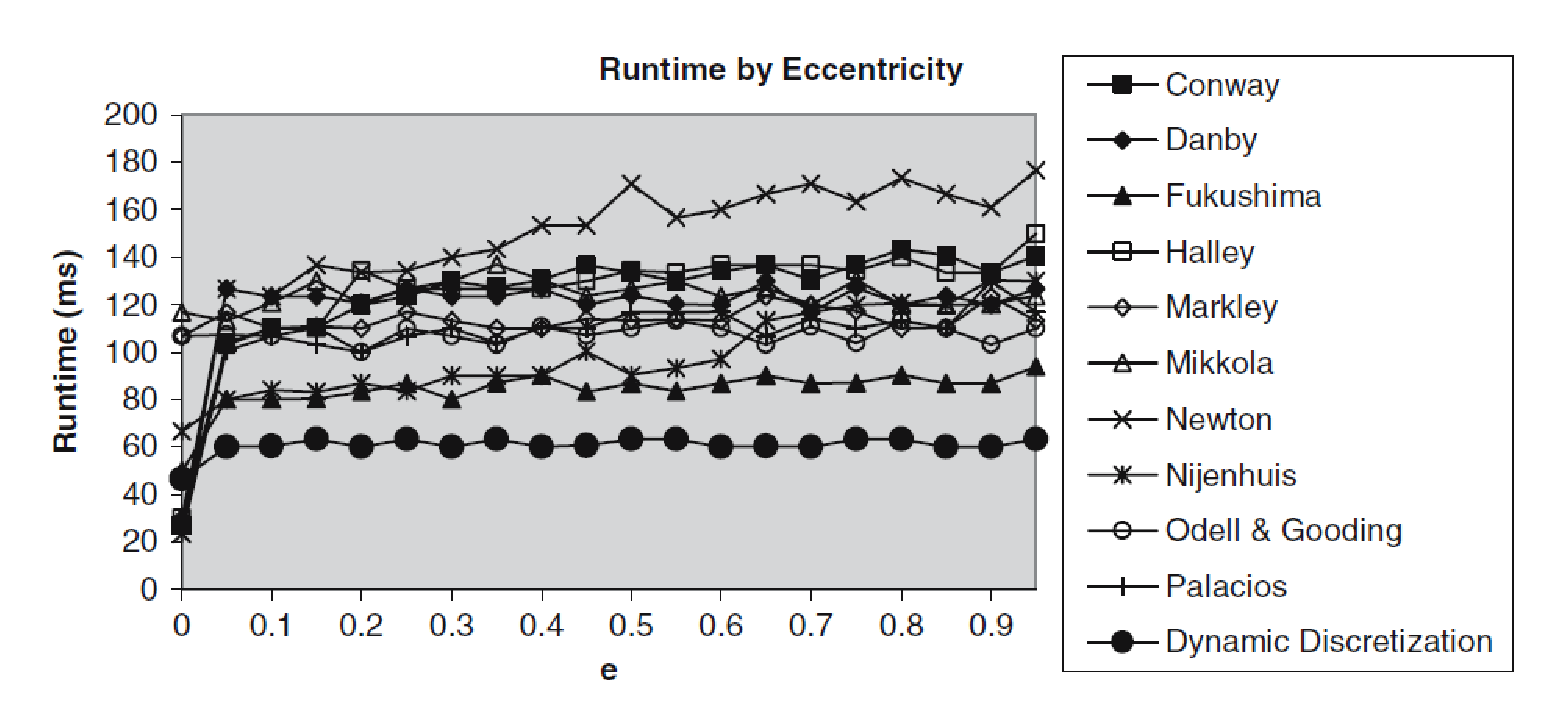
\includegraphics[scale=0.4]{me20b050.eps}
        \end{center}
        \caption{Runtime varying with eccentricity}
        \label{fig: runtime}
\end{figure}

Figure \ref{fig: runtime} shows us that Halley's method does certainly do better than the Newton-Rhapson method but recent techniques such as Dynamic Discretization are far more efficient

\newpage
